\chapter{Geometric Applications of Integrals}
Now that we are much better at the process of antidifferentiation, we apply integrals to the classic problems of geometry.  We find lengths, areas, volumes, and centers of mass.  Before we begin, we state L'Hospital's Rule, which will assist in computing areas of unbounded regions.

\section{L'Hospital's Rule}\label{LHR}

L'Hospital's Rule (LHR) allows us to evaluate \deriv{indeterminate limits} of the form \LHR{$\frac{0}{0}$ or $\frac{\infty}{\infty}$}.  It says that in either of these cases, we can simply differentiate the numerator and the denominator and try again.  

\begin{theorem}{L'Hospital's Rule} Let $c$ be a real number, $\infty$, or $-\infty$.  If $\lim_{x \rightarrow c}f(x)=\lim_{x \rightarrow c}g(x)=0$ or  $\lim_{x \rightarrow c}f(x)=\lim_{x \rightarrow c}g(x)=\infty$, then 
 $$ \lim_{x \rightarrow c}\frac{f(x)}{g(x)}=\lim_{x \rightarrow c}\frac{f'(x)}{g'(x)}$$
\end{theorem}

For the moment, we will just accept LHR and use it.  In Section \ref{EvalLHR}, we will prove LHR using power series.  Notice that here we do not differentiate with a Quotient Rule.  We instead simply differentiate the top and differentiate the bottom.

\begin{example}{Sine of a Small Angle}
\begin{wrapfigure}{r}{0.3\textwidth}
    	\centering
		\includegraphics[width=0.3\textwidth]{ChapterGeom/Figures/GAI-smallAngle}
        \caption*{Small angle $\theta$ verusus $\sin(\theta).$}
\end{wrapfigure}

 Consider the following limit: $$ \lim_{x\rightarrow 0}\frac{\sin(\theta)}{\theta}$$
It is indeterminate of the form $\frac{0}{0}$.  Thus it is valid to apply LHR. \begin{align*}
\lim_{x\rightarrow 0}\frac{\sin(\theta)}{\theta} &=\lim_{x\rightarrow 0}\frac{\left(\sin(\theta)\right)'}{\left(\theta\right)'} \\
&=\lim_{x\rightarrow 0}\frac{\cos(\theta)}{1} \\
&=1
\end{align*}
    
    
\end{example}
\begin{exercise}{Interpreting the Above Example \Coffeecup}
Since the ratio of $\sin(\theta)$ to $\theta$ approaches 1 as $\theta$ gets small, it would be appropriate to say the following (fill in the blanks):
\begin{center}
\emph{For small values of $\theta$, \underline{\hspace{1in}}$\approx$\underline{\hspace{1in}}.}
\end{center}
\end{exercise}
Note that this property comes up frequently in physics!  For example, when modeling the motion of a mass hanging from a spring, Hooke's Law tells us that force is proportional to displacement.  We use the same model to describe motion of a pendulum, even though in that case force is not technically proportional to displacement, but rather the \emph{sine} of displacement.  Why can we throw away the sine?  It is because for small displacements, the sine of the displacement is roughly equal to the displacement!
\begin{exercise}{Practice with LHR \Coffeecup \Coffeecup}
Evaluate the following limits using L'Hospital's Rule. In each case, justify why it is ok to use it!
\begin{itemize}
\item $ {\underset{x \rightarrow \infty}{\lim}}\hspace{.1in}\frac{x^2 }{ 2^x} $
\solushun{$${\lim_{x \rightarrow \infty}}\frac{x^2 }{ 2^x} = \frac{\infty}{\infty}$$Since we have the form $\frac{\infty}{\infty}$ we can use LHR.
$${\lim_{x \rightarrow \infty}}\frac{x^2 }{ 2^x}={\lim_{x \rightarrow \infty}}\frac{2x}{2^x\ln2}$$
Keep going:
$${\lim_{x \rightarrow \infty}}\frac{2x}{2^x\ln2}={\frac{1}{\ln2}\lim_{x \rightarrow \infty}}\frac{2}{2^x\ln2}={\frac{1}{(\ln2)^2}\lim_{x \rightarrow \infty}}\frac{1}{2^{x-1}}=0$$
}{1in}
\item $ {\underset{x \rightarrow 2}{\lim}}\hspace{.1in}\frac{x-2 }{ \sin(\pi x)} $
\solushun{
$${\lim_{x\to2}}\frac{x-2}{\sin(\pi x)}=\frac{0}{0}$$
So LHR is justified.
$${\lim_{x \to 2}}\frac{x-2}{\sin(\pi x)}={\lim_{x\to2}}\frac{\frac{\dif}{\dif x}(x-2)}{\frac{\dif}{\dif x}\sin(\pi x)}=\frac{1}{\pi\cos(\pi x)}=\frac{1}{\pi}$$
}{1in}
\item $ {\underset{x \rightarrow \infty}{\lim}}\hspace{.1in}\frac{ \arctan(x)-\pi/2 }{ \sin(1/x)} $
\solushun{$${\lim_{x\to\infty}}\frac{\arctan(x)-\pi/2}{\sin(1/x)}=\frac{0}{0}$$
So LHR is justified.
\begin{align*}
{\lim_{x\to\infty}}\frac{\arctan(x)-\pi/2}{\sin(1/x)}&={\lim_{x\to\infty}}\frac{\frac{\dif}{\dif x}(\arctan(x)-\pi/2)}{\frac{\dif}{\dif x}\sin(1/x)}={-\lim_{x\to\infty}}\frac{\frac{1}{x^2+1}}{\frac{1}
{x^2}\cos(1/x)}\\
&={-\lim_{x\to\infty}}\frac{x^2}{(x^2+1)\cos(1/x)}=-\frac{\infty}{\infty}\\
\text{One more time}\\
&={-\lim_{x\to\infty}}\frac{2x}{2x\cos(1/x)+\sin(1/x)+\frac{1}{x^2}\sin(1/x)}=-\frac{\infty}{\infty}\\
\text{And again}\\
&={-\lim_{x\to\infty}}\frac{2}{2\cos(\frac{1}{x})+2x(-\frac{1}{x^2}\sin(\frac{1}{x}))+\frac{1}{x^2}\cos(\frac{1}{x})-\frac{1}{x^4}\cos(\frac{1}{x})}\\
&=1
\end{align*}}{1in}
\end{itemize}
\AnswerKeyEntry{The limits are 0, $1/\pi$, and -1. }
\end{exercise}
\subsection{Other Indeterminate Forms}
There are many \LHR{other indeterminate forms} besides just $\frac{0}{0}$ and $\frac{\infty}{\infty}$.  Others that come up include: 
\begin{itemize}
\item $0\cdot \infty$
\item $0^0$
\item $1^\infty$
\item $\infty-\infty$
\end{itemize}
Often these other forms can be rearranged algebraically to become $\frac{0}{0}$ or $\frac{\infty}{\infty}$.  After this rearrangement, they can then be evaluated with LHR (or perhaps the algebra itself resolves the indeterminate form and LHR will not be needed).  Common helpful strategies include:

\begin{itemize}
\item Multiplying the top and bottom of the limit by the same expression (especially the conjugate of an expression involving a radical).
\item Taking $e$ to the $\ln$ of the limit.
\item Rewriting a product as a fraction via $a\cdot b = \frac{b}{\frac{1}{a}}$.
\end{itemize}
\begin{example}{Rewriting a Different Indeterminate Form}
 Consider the function $\sin(x)^{\tan(x)}$.  As $x$ approaches $\frac{\pi}{2}$ from the left, the function takes on the indeterminate form $1^\infty$.  Thus, we try the second strategy described above, where we take $e$ to the $\ln$ of the limit.  Proceeding:
 \begin{align*}
 \lim_{x\rightarrow \pi/2^-}\sin(x)^{\tan(x)}&= \lim_{x\rightarrow \pi/2^-}e^{\ln\left(\sin(x)^{\tan(x)}\right)}\\
 &=\lim_{x\rightarrow \pi/2^-}e^{\tan(x)\ln\left(\sin(x)\right)}\\
 \end{align*}
 
\begin{wrapfigure}{r}{0.3\textwidth}
 \begin{center}
 	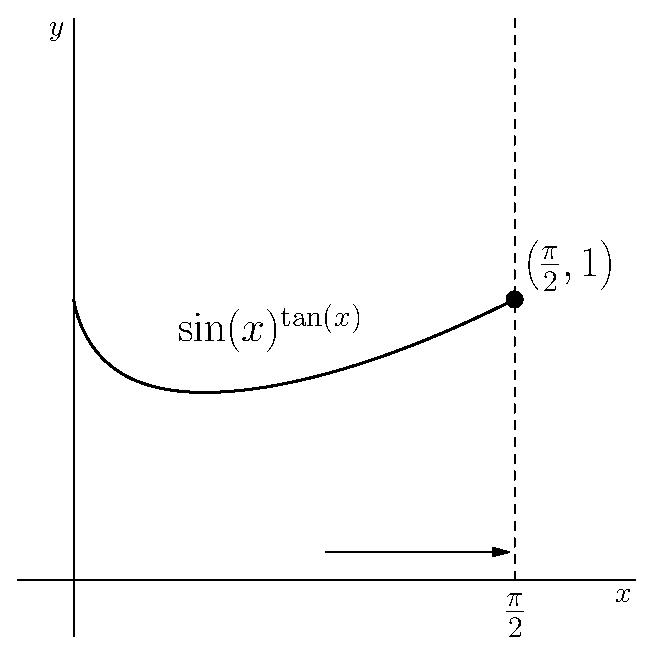
\includegraphics[width=0.3\textwidth]{ChapterGeom/Figures/LHR-SinetoTan}
 \end{center}
\end{wrapfigure}

Notice the exponent is now the indeterminate form $0\cdot\infty$.  Since the exponential function is continuous, we can move the limit inside and use LHR!
\begin{align*}
 \lim_{x\rightarrow \pi/2^-}\sin(x)^{\tan(x)}
 &=\lim_{x\rightarrow \pi/2^-}e^{\tan(x)\ln\left(\sin(x)\right)}\\
 &=e^{\lim_{x\rightarrow \pi/2^-}\left(\tan(x)\ln\left(\sin(x)\right)\right)}\\
 &=e^{\lim_{x\rightarrow \pi/2^-}\left(\frac{\ln\left(\sin(x)\right)}{\cot(x)}\right)}\\
 &=e^{\lim_{x\rightarrow \pi/2^-}\left(\frac{\left(\ln\left(\sin(x)\right)\right)'}{\left(\cot(x)\right)'}\right)}\\
 &=e^{\lim_{x\rightarrow \pi/2^-}\left(\frac{\frac{\cos(x)}{\sin(x)}}{-\csc^2(x)}\right)}\\
 &=e^{\lim_{x\rightarrow \pi/2^-}\left(-\cos(x)\sin(x)\right)}\\
 &=e^{-0\cdot 1}\\
 &=1
 \end{align*}
\end{example}
\begin{exercise}{Identifying LHR \Coffeecup}
In the example above, circle the exact step where LHR was applied.  Why was it ok to use LHR on that step?  Write a short sentence to explain.
\solushun{The steps from $e^{\lim_{x\rightarrow \pi/2^-}\left(\frac{\ln\left(\sin(x)\right)}{\cot(x)}\right)}$ to $e^{\lim_{x\rightarrow \pi/2^-}\left(\frac{\frac{\cos(x)}{\sin(x)}}{-\csc^2(x)}\right)}$. This was justified because $\lim_{x\to\pi/2^-}\ln(\sin(x))=\ln(1)=0$ and $\lim_{x\to\pi/2^-}\cot(x)=0$ also.\\}{0in}
\end{exercise}
\begin{exercise}{Rewriting \Coffeecup \Coffeecup \Coffeecup}
Utilize these strategies to rewrite the limits below as $\frac{0}{0}$ or $\frac{\infty}{\infty}$ and then evaluate.  Note that some of these may need LHR after rewriting and some may not!
\begin{itemize}
\item $  {\underset{x \rightarrow \infty}{\lim}}\hspace{.1in} x\cdot \sin (1/x) $
\solushun{\begin{align*}
\lim_{x\to\infty}x\cdot\sin(1/x)&=\lim_{x\to\infty}\frac{\sin (1/x)}{\frac{1}{x}}\\
&=\lim_{x\to\infty}\frac{\left(\sin (1/x)\right)'}{\left(\frac{1}{x}\right)'}\\
&=\lim_{x\to\infty}\frac{-\frac{1}{x^2}\cos(1/x)}{\frac{1}{x^2}}\\
&=\lim_{x\to\infty}\cos(1/x)=1
\end{align*}}{2in}
\item $  {\underset{x \rightarrow \infty}{\lim}}\hspace{.1in}  x - \sqrt{x^2+4x+3} $
\solushun{We actually don't need LHR for this one.
\begin{align*}
\lim_{x\to\infty}x-\sqrt{x^2+4x+3}&=\lim_{x\to\infty}\left(x-\sqrt{x^2+4x+3}\right)\cdot\frac{x+\sqrt{x^2+4x+3}}{x+\sqrt{x^2+4x+3}}\\
&=\lim_{x\to\infty}\frac{x^2-x^2-4x-3}{x+\sqrt{x^2+4x+3}}\\
&=\lim_{x\to\infty}\frac{-4x-3}{x+\sqrt{x^2+4x+3}}\\
&=\lim_{x\to\infty}\frac{-4-\frac{3}{x}}{1+\sqrt{1+\frac{4}{x}+\frac{3}{x^2}}}\\
&=\frac{-4}{1+\sqrt{1}}=\frac{-4}{2}=-2\\
\end{align*}}{2in}
\item $ \underset{x \rightarrow \infty}{\lim}\hspace{.1in}  \left(1+ \frac{1}{x} \right) ^x $ ({\bf Note: } This limit is often taken as the definition of the constant you get here!)
\solushun{Rewrite this as $e^{x\ln\left(1+\frac{1}{x}\right)}$
Then the limit can be moved into the exponent and resolved:
\begin{align*}
\lim_{x\to\infty}e^{x\ln\left(1+\frac{1}{x}\right)}=&e^{\lim_{x\to\infty}x\ln\left(1+\frac{1}{x}\right)}\\
=&e^{\lim_{x\to\infty}\frac{\ln\left(1+\frac{1}{x}\right)}{\frac{1}{x}}}\\
\text{Now apply LHR}\\
=&e^{\lim_{x\to\infty}\frac{\frac{1}{1+\frac{1}{x}}\cdot -x^{-2}}{-x^{-2}}}\\
=&e^{\lim_{x\to\infty}\frac{x}{x+1}}\\
\text{Apply LHR again}\\
=&e^{1}=e\\
\end{align*}}{2in}
\end{itemize}
\AnswerKeyEntry{The limits are $1$, $-2$, and $e$. }
\end{exercise}

\begin{exercise}{Polyexposaurus \Coffeecup \Coffeecup \Coffeecup}
\begin{itemize}
\item Any positive real number raised to the zero is...
\solushun{1\\}{.5in}
\item Zero raised to any positive real number is...
\solushun{0\\}{.5in}
\item So, what is $  {\underset{x \to 0^+}{\lim}}  x^x $? 
\solushun{\begin{align*}
\lim_{x\to0^+}x^x&=e^{\lim_{x\to0^+}x\ln x}\\
\lim_{x\to0^+}x^x&=e^{-\lim_{x\to0^+}\frac{\ln x}{\frac{1}{x}}}\tag{Goes to $\frac{-\infty}{\infty}$ so we factor out $-1$}\\
\lim_{x\to0^+}x^x&=e^{-\lim_{x\to0^+}\frac{\frac{1}{x}}{-\frac{1}{x^2}}}\\
\lim_{x\to0^+}x^x&=e^{\lim_{x\to0^+}x}\\
\lim_{x\to0^+}x^x&=e^{0}=1\\
\end{align*}}{2in}
\end{itemize}
\AnswerKeyEntry{The results are 1, 0, and 1.}
\end{exercise}

Be careful when using LHR to only apply it in the two indeterminate forms specified above.  Applying LHR to an expression that is not either $\frac{0}{0}$ or $\frac{\infty}{\infty}$ will most likely produce incorrect results.  

\begin{exercise}{L'Urgent Care \Coffeecup \Coffeecup }
Consider the following limit.
$$ {\lim_{x \to \pi }}  \frac{\sin(x)}{x} $$
\begin{itemize}
\item Why would it be wrong to apply LHR to the above limit?
\solushun{The denominator does not approach 0\\}{.5in}
\item  What do you get if you blindly apply LHR?
\solushun{$$\lim_{x\to\pi}\cos(x)=1$$}{.5in}
\item  What should the limit actually be?
\solushun{$$\lim_{x\to\pi}\sin(x)\cdot\frac{1}{x}=0\cdot\frac{1}{\pi}=0$$}{.5in}
\end{itemize}
\end{exercise}

\subsection{Growth Orders}\label{tomato} 

\growthorder{LHR} is often used for comparing \LHR{growth orders} of functions.  To compare the growth orders of functions, we take the limit of their ratio as $x$ approaches infinity and then see if the ratio approaches zero, a nonzero constant, or infinity to see which is growing faster.  More formally:

\begin{definition}{Growth Order}\label{tomahto}

Let $f(x)$ and $g(x)$ be functions on the real numbers. 
\begin{itemize}
\item If $\lim_{x\rightarrow \infty}\frac{f(x)}{g(x)}=0$, then $g(x)$ has \emph{larger growth order} than $f(x)$. 
\item If $\lim_{x\rightarrow \infty}\frac{f(x)}{g(x)}$ is a nonzero constant, then $f(x)$ and $g(x)$ have the \emph{same growth order}. 
\item If $\lim_{x\rightarrow \infty}\frac{f(x)}{g(x)}=\infty$, then $f(x)$ has \emph{larger growth order} than $g(x)$. 
\end{itemize}
\end{definition}
\begin{exercise}{Comparing the Growth Orders of Two Lines \Coffeecup \Coffeecup}
Consider the following two linear functions: \begin{align*}
f(x)&=6x+1\\
g(x)&=2x-1
\end{align*}
Fill out the table below to study some of their values and corresponding ratios.  Use decimal approximations for values that aren't integers.  \begin{center}
\begin{tabular}{|c||c|c|c|c|c|} \hline
$x$ & 1 & 10 & 100 & 1,000 & 10,000 \\ \hline
& & & & & \\
$f(x)$ & & & & & \\
& & & & & \\
$g(x)$ & & & & & \\
& & & & & \\
$f(x)/g(x) $ & & & & & \\
& & & & & \\ \hline
\end{tabular}
\end{center}
\solushun{ \begin{center}
\begin{tabular}{|c||c|c|c|c|c|} \hline
$x$ & 1 & 10 & 100 & 1,000 & 10,000 \\ \hline
& & & & & \\
$f(x)$ & 7& 61& 601& 6001& 60001\\
& & & & & \\
$g(x)$ & 1& 19& 199& 1999& 19999\\
& & & & & \\
$f(x)/g(x)$ & 7& 3.2105& 3.0201& 3.0020& 3.0002\\
& & & & & \\ \hline
\end{tabular}
\end{center}}{0in}
\begin{itemize}
\item From the table, does it appear that the ratio $f(x)/g(x)$ is approaching zero, infinity, or a nonzero constant?
\solushun{It appears that the ratio approaches the constant 3\\}{.3in}
\item Use LHR to compute the limit $$\lim_{x\rightarrow \infty}\frac{f(x)}{g(x)} $$
How does it relate to the values in the data table? 
\solushun{\begin{align*}
\lim_{x\to\infty}\frac{f(x)}{g(x)} &=\frac{\infty}{\infty}\\
&=\lim_{x\to\infty}\frac{f'(x)}{g'(x)}\\
&=\lim_{x\to\infty}\frac{6}{2}=3
\end{align*}
It is the ratio of the leading coefficients.\\}{.3in}
\item See the above definition of Growth Order.  In this case, would you say $f$ and $g$ have the same growth order, or does one function have larger growth order than the other?
\solushun{Since 3 is a nonzero constant, the two have the same growth order.}{.3in}
\end{itemize}
\AnswerKeyEntry{Their ratio converges to 3 (both numerically in the table, and analytically as evaluated by LHR).  Since this is a nonzero constant, the two functions have the same growth order.}
\end{exercise}

The above calculation justifies why it is ok to talk about something having \emph{linear growth order} or \emph{growing linearly}.  Any two lines have the same growth order (ignoring vertical and horizontal), so it is perfectly well-defined to talk about linear growth even if the slope or intercepts of the lines being discussed are unknown.  

This concept comes up frequently in computer science when you try to measure the runtime of algorithms.  If $f(x)$ is the number of operations performed by an algorithm that is handed an input of size $x$, then a logarithmic growth order of $f(x)$ is generally more desirable than a linear growth order, which is more desirable than quadratic growth order, and so on.

\begin{exercise}{A Visual Representation of Growth Order \Coffeecup \Coffeecup \Coffeecup}

In each of the graphs below, there is a graph of $f(x)$ and a graph of $g(x)$.  Based on the graphs, do you expect that $f$ and $g$ have the same growth order, or is one larger?

\begin{tabular}{l c }
1. &
    \raisebox{\dimexpr-\height + 1.5ex\relax}{\includegraphics[width=250pt]{ChapterGeom/Figures/Prob1.eps}} \\
2. &
    \raisebox{\dimexpr-\height + 1.5ex\relax}{\includegraphics[width=250pt]{ChapterGeom/Figures/Prob2.eps}} \\
    3. &
    \raisebox{\dimexpr-\height + 1.5ex\relax}{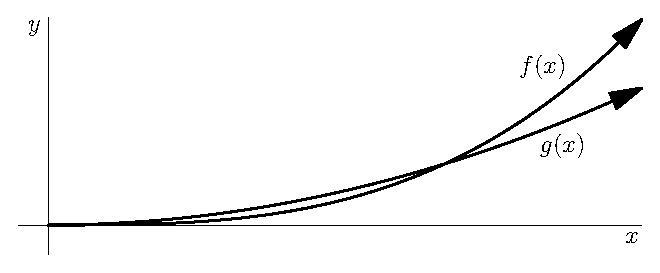
\includegraphics[width=250pt]{ChapterGeom/Figures/Prob3.eps}}
\end{tabular}

\AnswerKeyEntry{In the first and third, the ratio between $f$ and $g$ seems to grow without bound, so $f$ has larger growth order.  In the second, the ratio of $f$ to $g$ seems to always be right around 2.  Thus, they have the same growth order.}
\end{exercise}

\begin{example}{Logarithmic Growth Order}
\begin{wrapfigure}{r}{0.5\textwidth}
 \begin{center}
 	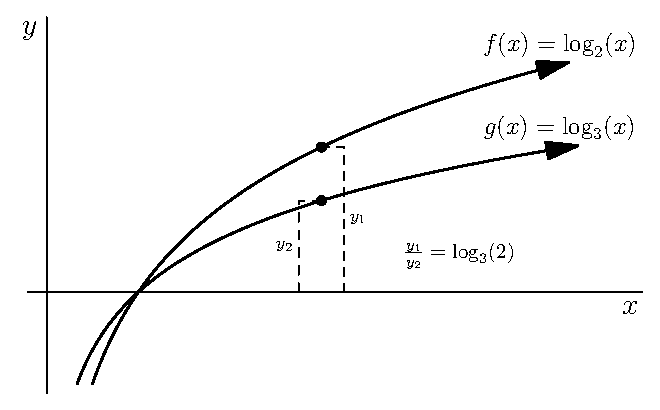
\includegraphics[width=0.5\textwidth]{ChapterGeom/Figures/LogGrowthOrder}
 \end{center}
\end{wrapfigure}
Here we compare the growth orders of the following logarithmic functions:
\begin{align*}
f(x)&=\log_2(x) \\
g(x)&=\log_3(x)
\end{align*}
Definition \ref{tomato}.\ref{tomahto}. shows that we should take the limit of their ratio and then see if we get zero, infinity, or a nonzero constant.

\begin{align*}
\lim_{x\to \infty}\frac{f(x)}{g(x)}&=\lim_{x\to \infty}\frac{\log_2(x)}{\log_3(x)}\\
&=\lim_{x\to \infty}\log_3(2) \\
&=\log_3(2)
\end{align*}
Since their ratio came out to a nonzero constant, we conclude that those two functions in fact have the same growth order (even though  the $y$-coordinate of $f(x)$ is always bigger).  By a similar calculation, we could observe that in fact any two logarithms have the same growth order regardless of what the base is!
\end{example}

\begin{exercise}{Race of the Turtles \Coffeecup \Coffeecup}
Rank the following functions by growth order from slowest to fastest by comparing their growth orders two at a time:
\begin{align*}
f(x)&=x {\ln} (x) \\
g(x)&=x^{1.1} \\
h(x)&=x\left( {\ln} (x) \right)^2
\end{align*}

\solushun{
Comparing $f(x)$ with $g(x)$:
\begin{align*}
\lim_{x\to\infty}\frac{x\ln(x)}{x^{1.1}}&=\lim_{x\to\infty}\frac{\ln(x)}{x^{0.1}}\\
&=\lim_{x\to\infty}\frac{x^{-1}}{0.1x^{-0.9}}\tag{By LHR}\\
&=\lim_{x\to\infty}\frac{x^{-0.1}}{0.1}=0
\end{align*}
So $g(x)$ has greater growth order than $f(x)$. Comparing $f(x)$ and $h(x)$:
\begin{align*}
\lim_{x\to\infty}\frac{x\ln(x)}{x\left(\ln(x)\right)^2}=\lim_{x\to\infty}\frac{1}{\ln(x)}=0
\end{align*}
So $h(x)$ has greater growth order than $f(x)$. Comparing $g(x)$ and $h(x)$:
\begin{align*}
\lim_{x\to\infty}\frac{x^{1.1}}{x\left(\ln(x)\right)^2}&=\lim_{x\to\infty}\frac{x^{0.1}}{\left(\ln(x)\right)^2}\\
&=\lim_{x\to\infty}\frac{0.1x^{-0.9}}{2\ln(x)x^{-1}}\tag{By LHR}\\
&=\frac{1}{20}\lim_{x\to\infty}\frac{x^{0.1}}{\ln(x)}\\
&=\frac{1}{20}\lim_{x\to\infty}\frac{0.1x^{-0.9}}{x^{-1}}\tag{By LHR again}\\
&=\lim_{x\to\infty}x^{0.1}=\infty
\end{align*}
So $g(x)$ has higher growth order than $h(x)$.
Then, the overall ranking is: $f(x),h(x),g(x)$.\\
}{2in}

\end{exercise}

\begin{exercise}{Exponential vs Polynomial \Coffeecup \Coffeecup \Coffeecup }
Explain why an exponential function will always have larger growth order than an polynomial function. 
\solushun{An exponential function $c^x$ will always have a larger growth order than any polynomial function because the derivative will always contain another $c^x$ term. That is $(c^x)'=c^x\ln(c)$. In the simplest case, $(e^x)'=e^x$. Thus, as long as $x>0$, the limit of any of the derivatives of an exponential function, $\lim_{x\to\infty}(c^x)^{(k)}$, with $k>0$ is always $\infty$.

A polynomial, on the other hand, either has derivatives that eventually become constant (if the power $n$ of a term $x^n$ is greater than 0), or which become successively smaller (if $n$ is less than 0). Thus, the polynomial's successive derivatives will eventually become less than that of an exponential function.\\

On the other hand, if $x<0$, the exponential function will always have a smaller growth order than any polynomial.\\}{2in}
\end{exercise}
